%\documentclass[12pt]{article}
%\usepackage[a4paper, margin=1in]{geometry} 
%\usepackage{graphicx} 
%\usepackage{hyperref}
%\usepackage{float}
%\usepackage{multicol}
%\usepackage[font=small, labelfont=bf]{caption}
%
%\begin{document}

%
% Homology at the sequence level
%
\subsection{Homology at the sequence level}
Constructing alignments can be useful to understand homology among different species. Finding homologies is important to reveal a common evolutionary ancestor.

%
% Evolution and homology
%
\subsubsection*{Evolution and homology}
All species are derived from a common ancestor at some point during the course of evolution.
 
\begin{figure}[H]
  \centering
      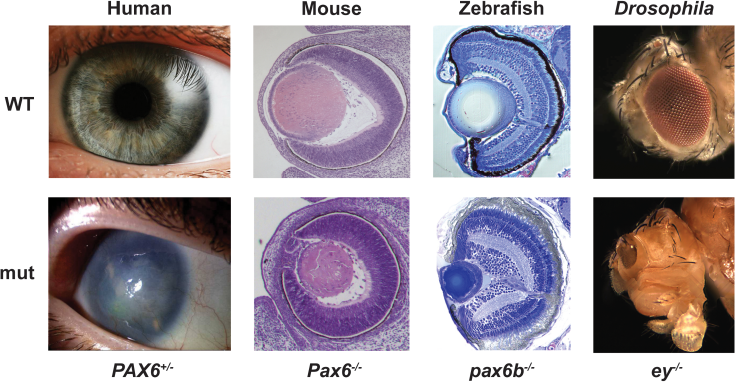
\includegraphics[width=0.5\textwidth]{fig03/PAX6_mutation.png}
  \caption{PAX6 alterations result in similar changes to eye morphology \newline (source: Washington et al, doi: 10.1371/journal.pbio.1000247 via \href{https://commons.wikimedia.org/w/index.php?curid=8626896}{Wikimedia Commons})}
\end{figure}

%
% Homologous and  analogous
%
\subsubsection*{Homologous and  analogous}
It is useful to check similarity at the molecular level because there are cases that analogous structures may not indicate homologous. 
\begin{figure}[H]
  \centering
      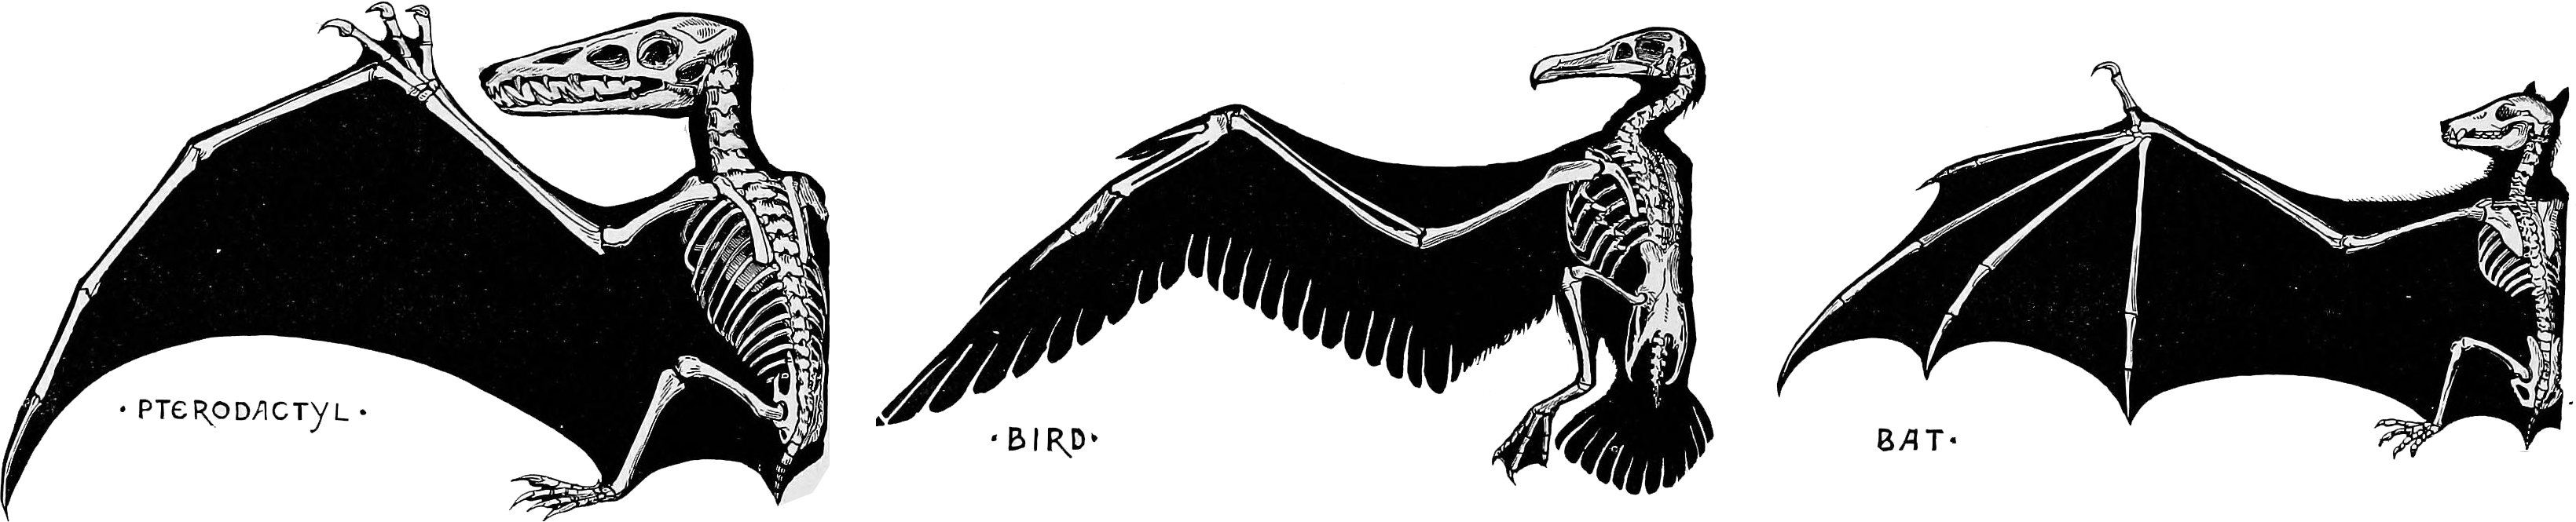
\includegraphics[width=0.5\textwidth]{fig03/analogous.png}
  \caption{Homologous and  analogous structures \newline (source: John Romanes, 1892, Darwin and after Darwin via \href{https://commons.wikimedia.org/w/index.php?curid=1324636}{Wikimedia Commons})}
\end{figure}

%
% Sequence homology
%
\subsubsection*{Sequence homology}
\begin{figure}[H]
  \centering
      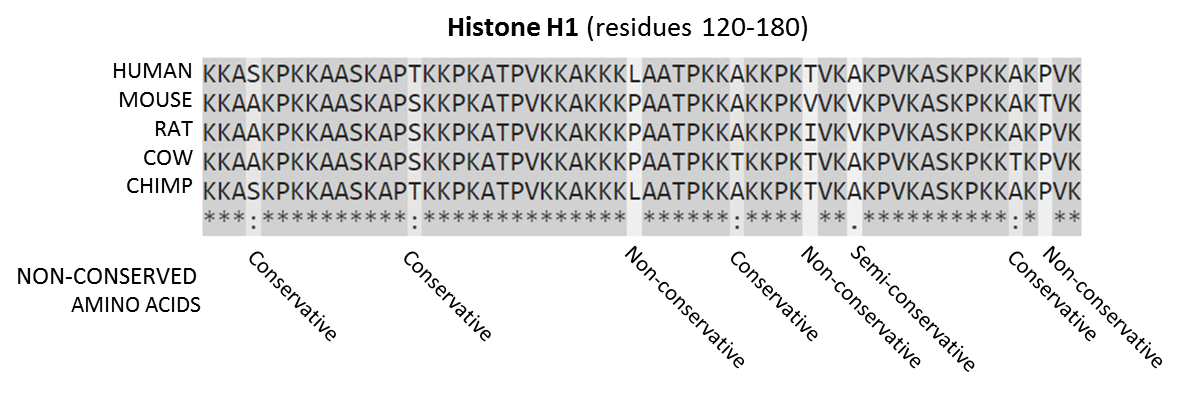
\includegraphics[width=0.75\textwidth]{fig03/histone_alignment.png}
  \caption{Multiple sequence alignment of histone sequences \newline (source: \href{https://commons.wikimedia.org/w/index.php?curid=37188728}{Shafee, Wikimedia Commons})}
\end{figure}

%
% Sequence homology
%
\subsubsection*{Evolution at the sequence level}
Sequence differences in DNA
\begin{itemize}
\item Substitution (a mismatch in alignment)
\item Insertion (a gap in alignment)
\item Deletion (a gap in alignment)
\item Inversion
\end{itemize}

\noindent
Sources of variations
\begin{itemize}
\item Mutation
\item Recombination
\item Insertional mutagenesis
\item ...
\end{itemize}

\noindent
A mutation of the third nucleotide in a codon often does not affect which amino acid is synthesized.
\begin{itemize}
\item GCU $\rightarrow$ Ala (Alanine)
\item GCC $\rightarrow$ Ala (Alanine)
\item GCA $\rightarrow$ Ala (Alanine)
\item GCG $\rightarrow$ Ala (Alanine)
\end{itemize}

\noindent
An amino acid can be replaced by a different amino acid that has similar properties in some cases.
\begin{itemize}
\item AUU, AUC, AUA $\rightarrow$ Ile (Isoleucine)
\item CUU, CUC, CUA $\rightarrow$ Leu (Leucine)
\end{itemize}

%
% Extension of global alignment
%
\subsubsection*{Extension of global alignment with DP}

\begin{itemize}
\item Score matrix \\
DNA, RNA, and protein

\item Gap penalty \\
Linear, affine, and constant
\end{itemize}

\bigskip 

%\end{document}
